%\usebackgroundtemplate{%             declare it
%	\tikz[overlay,remember picture] \node[opacity=1, at=(current page.center)] {
%		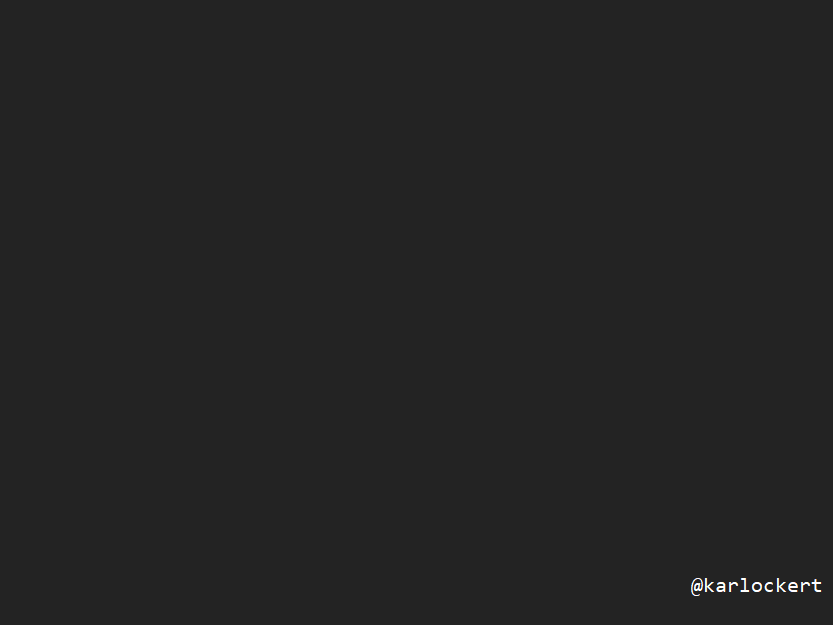
\includegraphics[height=\paperheight]{img/bakgrunn.png}};}

\begin{frame}[noframenumbering, plain]
	\begin{block}{\color{white}\textbf{\Large{
		Linear response - The Kubo formula
			}}}
		\vspace{-10pt}\rule{\textwidth}{0.5pt}
		\color{white}
			In linear response theory, the Kubo formula relates a non-equilibrium quantum property with its value at equilibrium. 
			The setup is as follows; start with a qantity $O$ you want to measure, and a time independent Hamiltonian $H_0$.
			Then, at time $t = t_0$, a time-dependent (small) perturpation $H'$ is added to the system. 
			The Kubo formula states that the (now time-dependent) observed value for $O$ will be (to linear order)

	\end{block}
	{\large
		
		\begin{equation*} 
			\ev*{O(t)} = \ev*{O}_{0} - i \int_{t_0}^{t}\dd{t'}\ev{\comm*{\hat{O}(t)}{\hat{H}'(t')}}_{0}.
		\end{equation*}
	}

	\begin{block}{}
	\color{white}
	
		This can be highly useful, since it can give relatively good approximations to what will happen when one suddenly makes small changes to the physical system.
		(Example: how conductivity changes when suddenly changing a weak magnetic field)
		
	\end{block}
	

\end{frame}